\begin{figure}[H]
\centering
\shorthandoff{<>}
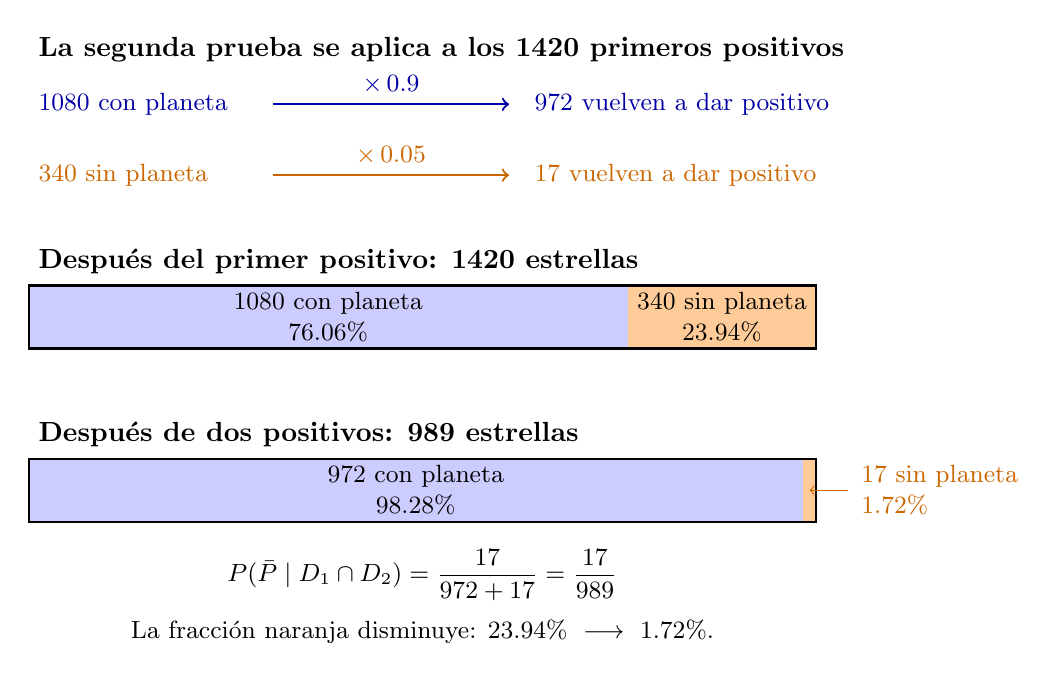
\begin{tikzpicture}[font=\small]
  \node[anchor=west,font=\bfseries] at (0,0.7)
    {La segunda prueba se aplica a los 1420 primeros positivos};
  \node[anchor=west,text=blue!65!black] at (0,0) {1080 con planeta};
  \draw[->,thick,blue!65!black] (3.1,0) -- (6.1,0)
    node[midway,above] {$\times\,0.9$};
  \node[anchor=west,text=blue!65!black] at (6.3,0) {972 vuelven a dar positivo};
  \node[anchor=west,text=orange!80!black] at (0,-0.9) {340 sin planeta};
  \draw[->,thick,orange!80!black] (3.1,-0.9) -- (6.1,-0.9)
    node[midway,above] {$\times\,0.05$};
  \node[anchor=west,text=orange!80!black] at (6.3,-0.9) {17 vuelven a dar positivo};

  \node[anchor=west,font=\bfseries] at (0,-2) {Después del primer positivo: 1420 estrellas};
  \fill[blue!20] (0,-3.1) rectangle ({10*1080/1420},-2.3);
  \fill[orange!40] ({10*1080/1420},-3.1) rectangle (10,-2.3);
  \draw[thick] (0,-3.1) rectangle (10,-2.3);
  \node[align=center] at ({5*1080/1420},-2.7) {1080 con planeta\\$76.06\%$};
  \node[align=center] at ({5+5*1080/1420},-2.7) {340 sin planeta\\$23.94\%$};

  \node[anchor=west,font=\bfseries] at (0,-4.2) {Después de dos positivos: 989 estrellas};
  \fill[blue!20] (0,-5.3) rectangle ({10*972/989},-4.5);
  \fill[orange!40] ({10*972/989},-5.3) rectangle (10,-4.5);
  \draw[thick] (0,-5.3) rectangle (10,-4.5);
  \node[align=center] at ({5*972/989},-4.9) {972 con planeta\\$98.28\%$};
  \draw[->,orange!80!black] (10.4,-4.9) -- ({5+5*972/989},-4.9);
  \node[anchor=west,align=left,text=orange!80!black] at (10.45,-4.9)
    {17 sin planeta\\$1.72\%$};

  \node[align=center] at (5,-6.25)
    {$\displaystyle P(\bar P\mid D_1\cap D_2)=\frac{17}{972+17}=\frac{17}{989}$\\[6pt]
    La fracción naranja disminuye: $23.94\%\ \longrightarrow\ 1.72\%$.};
\end{tikzpicture}
\shorthandon{<>}
\caption{Confirmación secuencial bajo independencia condicional dado el estado real de la estrella. Se conservan el $90\%$ de los positivos con planeta y el $5\%$ de los positivos sin planeta. Las frecuencias son esperadas para la misma población ilustrativa de 8000 estrellas. Cada barra representa el $100\%$ de su propio grupo: sus anchos comparan proporciones, no cantidades de estrellas.}
\label{fig:bayes-confirmacion}
\end{figure}